\chapter{Opportunistic Relaying}
\label{chap:opp_relay}

\section{Background}
Wireless network providers are under tremendous pressure to deliver unprecedented amounts of data to a variety of mobile devices. A powerful concept that has only gained limited traction in practice has been the concept of opportunistic networks whereby nodes opportunistically communicate with each other when in range to augment or overcome existing wireless systems. Although opportunistic networking has received more attention as of late with the rise of various point-to-point technologies (WiFiDirect, LTEDirect) directly embedded in user devices, traction in terms of significant adoption remains elusive as the mere existence of point-to-point wireless technology is insufficient.  Rather, infrastructure support (albeit at a software or protocol level) is still required that is impeded by the lack of shared, longitudinal data taking a serious look at the potential for opportunistic relaying amongst actual mobile device users to justify said investment in infrastructure. The actual gathering of said data though is in and of itself quite difficult, requiring one to overcome numerous issues with respect to privacy, cost, scale, and quite simply the amenability of the device to acquire said data. Thus, in the absence of real data and the difficulty in acquiring such data, opportunistic networking research has largely espoused synthetic or theoretical explorations of user mobility.  In this Chapter, we demystify the opportunities that exist for opportunistic relaying by bridging the gap with our large scale dataset. 

\section{Related Work}\label{sec:related_work}
The notion of what constitutes an \emph{opportunistic communication} encompasses a wide variety of research and standardization efforts within the networking community.  From the more traditional perspective, opportunistic relaying represents wireless nodes taking advantage of emergent opportunities to relay data towards its eventual destination originally espoused by~\cite{laneman2004cooperative} and expanded up by numerous others \cite{bletsas2006simple,lu2009design,bahl2009opportunistic}.  More recently, considerable efforts have emerged where IEEE 802.11-based networks (WiFi) are viewed through an opportunistic viewpoint, espousing the delay of packets to favor the potentially faster WiFi over the congested cellular link.  More aggressive variants include `Opp-Off' as proposed in~\cite{han2011mobile2} which intentionally delays the delivery of information over cellular networks and offload it through the `free' opportunistic communications. Similarly, in~\cite{dimatteo2011cellular}, another delay-tolerant network (DTN)-like architecture called `MADNet' is proposed by integrating WiFi networks and mobile-to-mobile Pocket Switched Networks (PSN) with cellular networks.   With the ability to leverage the availability of inexpensive 802.11, both Opp-Off and MADNet are able to conduct real-world experiments on live systems, albeit on a limited scale and time period.   

A key foundation for the evaluation of opportunistic networks arises from the characterization of inter-contact times 
~\cite{chaintreau2007impact,cai2008toward,lee2009slaw,karagiannis2010power,passarella2011characterising}. The work in \cite{chaintreau2007impact} was one of the first works to highlight the importance of inter-contact for studying opportunistic networks and analyze the features of aggregate inter-contact times. In the work of~\cite{cai2008toward,lee2009slaw}, the mobility models proposed for opportunistic networks aim at reproducing the aggregate power-law distributions.  The mobility models in turn provide powerful abstractions for the evaluation of various theoretical properties of opportunstic networks that is critical for understanding general limits of the overarching relay protocols.  In contrast from these studies on statistical patterns of human mobility, we focus on the analysis to take in not only the proximity into consideration but also other elements such as traffic needs and battery influences which have to the best of our knowledge, not explored in a unified manner in the literature. 

\section{Evaluating Practical Relaying}\label{sec:potential}

The dataset outlined in Chapter~\ref{chap:dataset} provides a fascinating opportunity to evaluate the actual prevalence with respect to opportunistic relaying in the `wild' evaluating not only the prevalence itself but when intra-study proximity is involved, significant explorations with respect to the mutual benefits of relaying or collaborative efforts.  For the purposes of evaluation, we are concerned with two types of opportunistic networking, namely relaying and collaboration.  In the first case of relaying, a mobile node ($MN_i$) might relay the traffic from mobile node ($MN_j$) when $MN_j$ has a weak / non-existent wireless signal or $MN_i$ has a good signal to a preferred wireless medium (ex. WiFi) while $MN_j$ does not.  In the second case of collaboration, $MN_i$ and $MN_j$ work together to overcome a lossy channel either by the use of striping across both nodes (ex. auxiliary relaying of TCP ACKs \cite{SteenkisteRelayACK}) or striping across different wireless mediums (WiFi + cellular).  Opportunistic communications would be provided through mobile-to-mobile communications (Bluetooth, WiFiDirect, LTEDirect). Both approaches to opportunistic relaying would require modifications to the wireless infrastructure as well as security concerns to establish any mobile-to-mobile communication which are beyond the scope of this paper.  Rather, we focus on the more fundamental question of \emph{does enough opportunity exist} and if so, \emph{is it of reasonable quality to make it worthwhile}?  

\begin{table*}[t] 
\caption{Framework for Evaluating Availability, Prevalence, Stability, Reciprocity} 
\centering
\begin{tabular}{l|p{3.5cm}|p{1.5cm}|p{11cm}}
\hline
\multicolumn{2}{c|}{Criteria} & \multicolumn{1}{c|}{Term} &\multicolumn{1}{c}{Description}  \\ 				
\hline
\hline  
\multirow{5}{*}{Availability}   & Sufficient Signal & $SS$ 	& `good signal' to indicate proximity  \\ 
\cline{2-4}		 			  & Symmetry & $Sym$		& Time when proximity is symmetric, has $SS$ vs. time powered on \\
\cline{2-4}		  		           & Diversity & $Div_n$	         & Time with at least $n$ nodes with $SS$ detected vs. time nodes detected \\ 
\cline{2-4}					  & Residual Battery & $RB$	& Time with proximity of other nodes with $SS$ and enough battery to do relaying vs. time with proximity \\

\hline  
\multirow{2}{*}{Prevalence}   & Time in Proximity & $TIP$ 	& Time with proximity vs. time powered on  \\ 
\cline{2-4}					  & Intercontact Time & $IT$	& Time between two successive contact/proximity periods \\
\cline{2-4}					  & Effective Utility & $EU$	& Time with proximity of other nodes with $SS$, $Sym$, traffic to send vs. time with traffic to send \\

\hline \multirow{4}{*}{Stability} 		& Duration & $D$			& Number of consecutive contact durations vs. instances of contact at $MN_i$ \\
\cline{2-4}			     			&  Node Strength & $NS$	&  Number of total appearances by $n$ most common peers \\
\cline{2-4}			     			&  Total Appearances & $TA$	& Number of appearances of a device vs. total device appearances at $MN_i$ \\
\cline{2-4}			     			&  Continuous Appearances & $CA$	& Number of consecutive appearances of a device vs. appearances of multiple days at $MN_i$ \\
\hline \multirow{4}{*}{Reciprocity}  & Need Service & $Serv$ & Time when no auxiliary WiFi is present and traffic demand exists vs. time powered on\\
\cline{2-4}	  		       		 & Offer Assistance & $Assist$ & Time ween detected with $SS$ vs. time powered on 	\\
\cline{2-4}					 & Ratio Need vs. Assist & $R_{NA}$ & Time of $Serv$ vs. Time of $Assist$ \\ 
\hline
\end{tabular}
\label{table:metrics} 
\end{table*}

To that end, we seek to answer the following questions in this section of the paper summarized in terms of metrics in Table \ref{table:metrics}:

\begin{itemize}
	\item \emph{Availability}: How is proximity defined and what criterion should exist to enable opportunistic communication with respect to inter-node communications?  What can be considered a `good' opportunistic link in terms of the underlying physical link quality and at what granularity is such data recorded? How does the residual battery influence the potential for relaying? 
	\item \emph{Prevalence}: What is the frequency that a mobile device detect other devices in proximity?  To what extent is the detection symmetric for intra-study participants?  How does the inter-contact times of nodes compare to prior work?  Do opportunities exist when needed (traffic demand) making them useful versus simply available?  
	\item \emph{Stability}: To what extent are discovered opportunities stable enough that an overarching security mechanism could complete or relevant data exchanges could take place?  Are there consistent patterns with regards to nodes appearing more common than others allowing expedited trust?   
	\item \emph{Reciprocity}: Even if opportunities are shown to be prevalent and stable, to what extent are the relationships likely to be reciprocal, namely both $MN_i$ and $MN_j$ will benefit on average equally in terms of both receiving assistance and giving assistance?  When energy is factored in as a consideration for nodes not being willing participants, does any sort of prevalence or reciprocality disappear?  Finally, reciprocality if it exists, does it exist exclusively in only longer-time scales or does it exist on reasonably short-time scales as well?    
\end{itemize}

For the wireless network, we first being by defining several key attributes of the data.  Each mobile node ($MN_i$) is considered to have a discrete set of samples at periodic intervals capturing the proximity of nearby nodes (Bluetooth), the signal strength from each detected Bluetooth node as received at $MN_i$, (ex. $MN_j \rightarrow MN_i$), each detected AP and also the signal strength for each AP as detected by $MN_i$ by virtue of the beacon signal strength.  Each time slot is assumed to be five minutes long (for the purposes of assessing if the phone was on or off) though durations of contact are calculated using per-minute measurements.  The term \emph{Good RSSI} refers to thresholds for RSSI values that indicate the potential for excellent performance although in practice such performance may vary.  Performance with respect to each node is normalized unless explicitly noted to the actual time that the phone was on (powered on, agent running) for that particular day or period. 

\subsection{Availability}
The first question to pose is how to define proximity. We begin with the most basic question with regards to the signal strength of discoverable Bluetooth devices and detected APs and further refine our queries to explore various aspects of availability through the Availability criterion of the APSR framework. 

\subsubsection*{Proximity}
We use Bluetooth as the proximity mechanism for multiple reasons.  First, the effective range of Bluetooth typically is on the order of 10m or less.  In contrast with other point-to-point technologies such as WiFiDirect and LTEDirect which have the potential for significantly longer ranges, Bluetooth in effect represents a minimum or floor to the potential for opportunistic communications as the various *Direct technologies would easily be able to cover the 10m effective range of Bluetooth.  Second, although Bluetooth is reasonably common amongst smart phones, the locking of a device as being discoverable is fairly uncommon, largely for reasons of security.  Despite the somewhat uncommon nature of discoverable Bluetooth (most devices require specific action to make themselves discoverable), a robust finding even with the limits of Bluetooth discoverability represents again a floor or minimum potential available.  Critically, the act of gathering Bluetooth discoverable devices is reasonably power efficient allowing one to gather available devices at a reasonable pace (with associated signal strength for Bluetooth) without pairing and while still having a reasonable device battery life for the study. 

Notably, the mere existence of the device being discoverable does not necessarily imply that the point-to-point link will be suitable for opportunistic communications.  Figure~\ref{fig:rssi} shows the ECDF of the Bluetooth RSSI values in different months and more than 60\% of the values are larger than -80dBm.  In particular, the data of July 2012 consider all the records including the Bluetooth devices outside the project and APs not under university control. Based on the work in ~\cite{polastre2005telos}, the RSSI value \emph{-80dBm} is used as a threshold to indicate good Bluetooth RSSI for direct mobile-to-mobile communication.  

\begin{figure}[tbp]
\centering 
{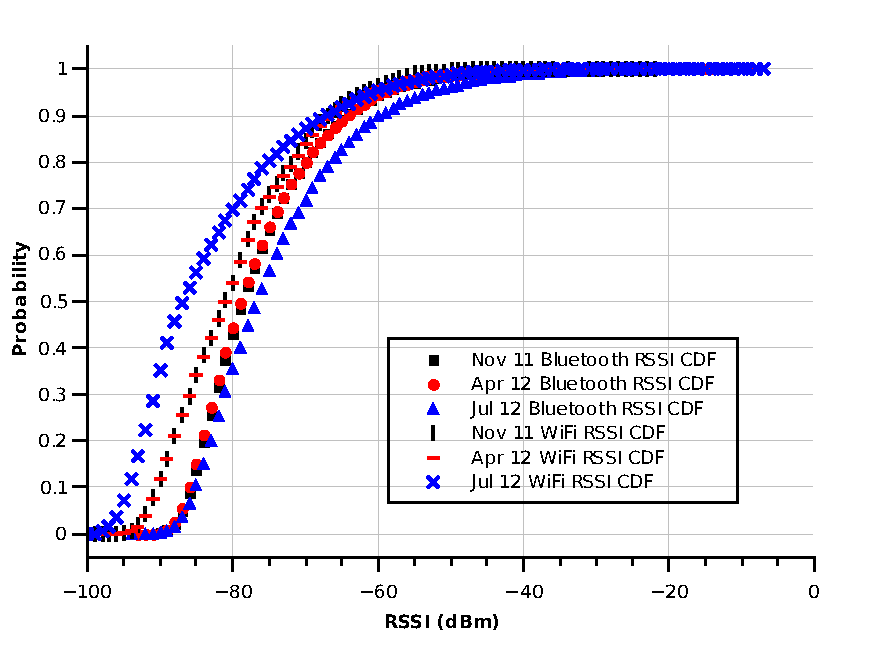
\includegraphics[width=3.5in]{graphs/rssi.pdf}}
\caption{Bluetooth and WiFi RSSI Values ECDF} 
\label{fig:rssi}
\end{figure} 

While Bluetooth is used in the first part of the section to assess proximity, to what extent could we infer proximity if we expanded our search to consider common detected WiFi APs.  For instance, in ~\cite{mcnett2005access}, WiFi signal strength is used to indicate proximity when two devices are associated to the same AP.  We further restrict the characterization to infer proximity if two mobile nodes detect two or more same access points.  Barring the two APs being situated nearly on top of one another (note that university APs are filtered down to disambiguate virtual APs), one can reasonably infer that two nodes sharing the same two or more APs could be in WiFiDirect and / or LTEDirect range. Figure~\ref{fig:bt_wifi_distribution} shows the ECDF of Bluetooth proximity percentage and WiFi proximity percentage. The percentage of time represents the percentage of time where an opportunity might exist for collaboration either within Bluetooth proximity or WiFi proximity. Interestingly, the WiFi result conveys less proximity than the noted Bluetooth proximity.  The discrepancy can be traced to one primary culprit, namely the poor signal reception of smartphone WiFi adapters as originally noted by \cite{liu:CellNet12}.  Notably when compared to reference laptops or tablets, the work in \cite{liu:CellNet12} notes a roughly 10 dBm signal penalty for the smartphone.  The net result is in addition to the detection of WiFi APs being hampered, reasonable placement of APs and auto-tuning of AP strength would result in significantly reduced probabilities of multiple mobile devices being able to detect one or more APs. In Figure~\ref{fig:wifi_fp_fn0}, we compare the results of WiFi proximity and Bluetooth proximity in April of 2012 and November of 2011. The false positive means the device detects other(s) in WiFi proximity which are not detected by Bluetooth proximity. On the other hand, the false negative means that the device does not detect some device in WiFi proximity but does detect the device in Bluetooth proximity. Notably, the false positive in the context of WiFi may not be a false positive but the false negative most certainly represents an incorrect result due to the aforementioned signal holes noted in \cite{liu:CellNet12}.  

\begin{figure}[tbp]
\centering 
{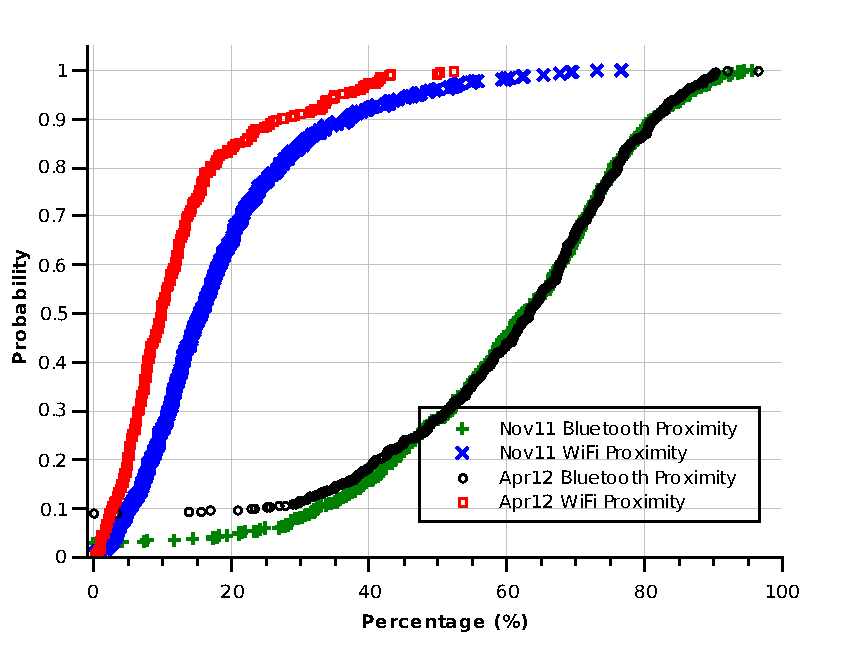
\includegraphics[width=3.5in]{graphs/bt_wifi_distribution_201204.pdf}}
\caption{Bluetooth Proximity and WiFi Proximity ECDF in April 2012} 
\label{fig:bt_wifi_distribution}
\end{figure} 

\begin{figure}[tbp]
\centering 
{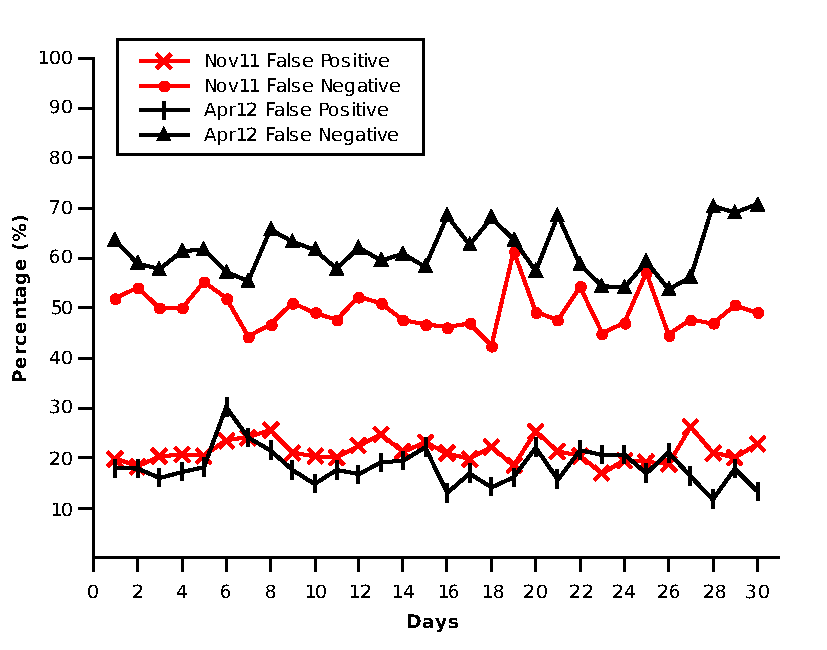
\includegraphics[width=3.5in]{graphs/wifi_falsenegative.pdf}}
\caption{Comparison of Bluetooth Proximity and WiFi Proximity} 
\label{fig:wifi_fp_fn0}
\end{figure} 

\subsubsection*{Symmetry}

Symmetry is defined as both nodes seeing each other in proximity. For WiFi proximity, such symmetry is 100\% based on its definition. However, for any two study participants in Bluetooth proximity, there exists the opportunity to determine if detection symmetric exists, namely do both nodes detect each other and even if both nodes detect each other, do both nodes have a `Good RSSI' to one another ($MN_i \rightarrow MN_j$ and vice versa)? In Figure~\ref{fig:daily_symmetric}, the symmetry of Bluetooth proximity within study with `Good RSSI' is illustrated by using the data in November 2011 and April 2012. Notably, roughly one third of the opportunities disappear due to the consideration of symmetry. Many reasons may cause the asymmetry such as environment inference and it is quite expectable in practice. 

\begin{figure}[tbp]
\centering 
{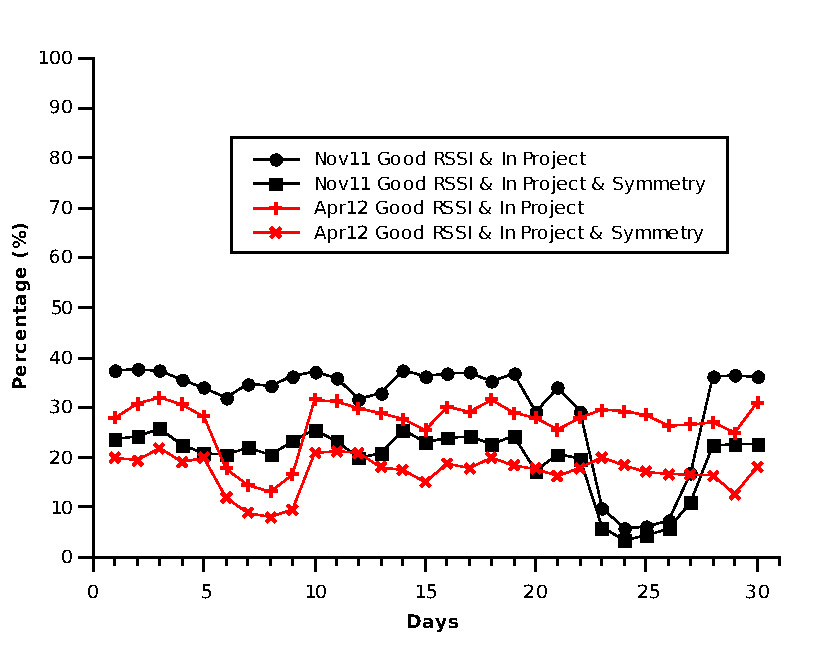
\includegraphics[width=3.5in]{graphs/daily_symmetric.pdf}}
\caption{Symmetry of Bluetooth Proximity} 
\label{fig:daily_symmetric}
\end{figure} 


\subsubsection*{Diversity}
While symmetry represents just one part of the puzzle, an related factor for the opportunity to be useful is with regards to the diversity of opportunities available.  Relaying selection plays little role when there exists only a single device to choose from for relaying.   Figure~\ref{fig:relay_num} shows the breakdown of detected devices in proximity through both Bluetooth and WiFi in April 2012 representing only cases where proximity occurred. In the figure, nearly 60\% of time has only one peer is detected among all the possible opportunistic time slots. Meanwhile, there is nearly 20\% of the time when two opportunities are detected and finally 20\% when three or more opportunities are detected. In Figure~\ref{fig:relay_num_diurnal}, more details about the number of detected devices in April 2012 is illustrated with a diurnal distribution across the same month breaking down only cases where proximity was detected, i.e. 50\% of daytime detections involved only a single device in the study. During the daytime, the chance to detect two or more devices in proximity is higher than other durations. Again, day time offers an increased potential for diversity in large part due to the increased mobility around the campus.  

\begin{figure}[tbp]
\centering 
{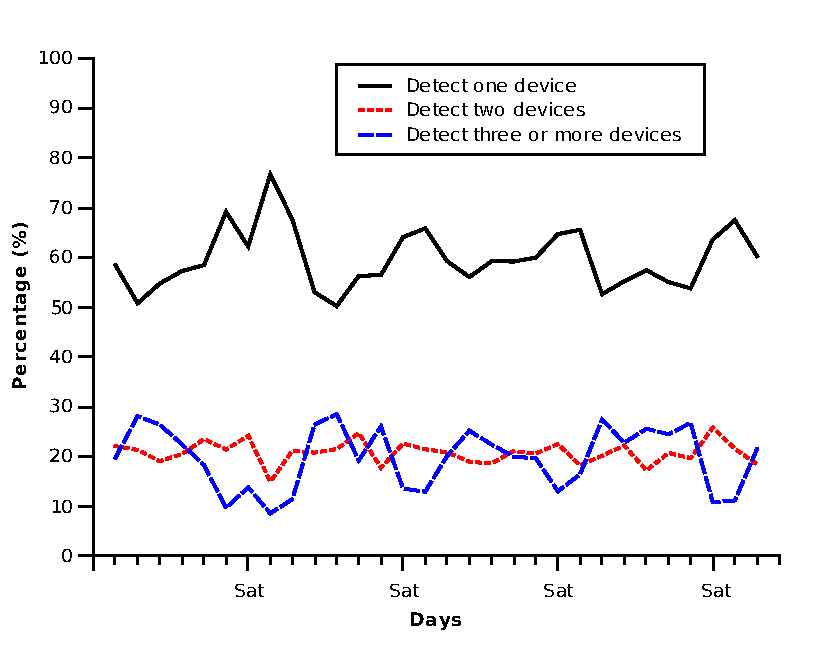
\includegraphics[width=3.5in]{graphs/relay_num.pdf}}
\caption{Distribution of Proximity Diversity (In-Study) in April 2012} 
\label{fig:relay_num}
\end{figure} 

\begin{figure}[tbp]
\centering 
{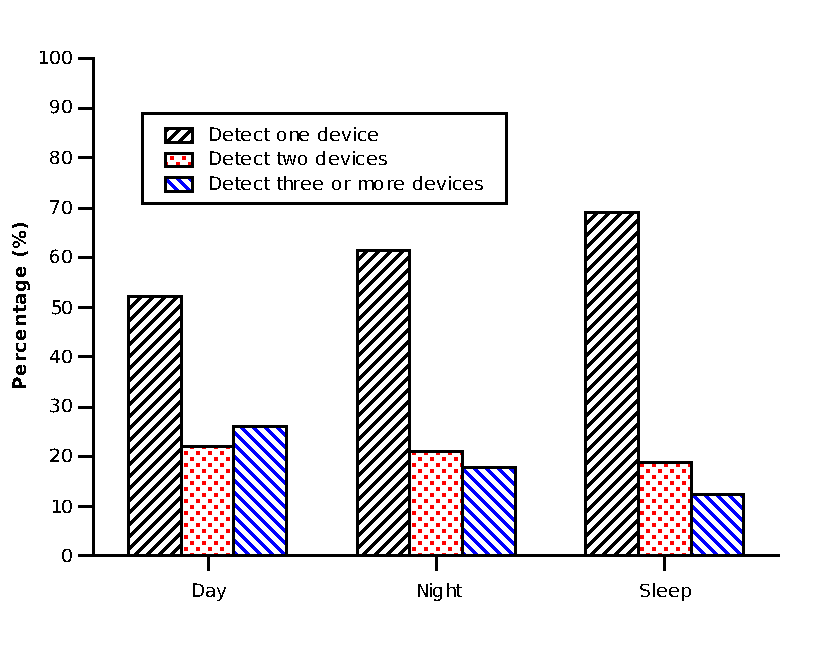
\includegraphics[width=3.5in]{graphs/relay_num_diurnal.pdf}}
\caption{Diurnal Distribution of Proximity Diversity in April 2012} 
\label{fig:relay_num_diurnal}
\end{figure} 

As mentioned before, it is fairly uncommon making the device Bluetooth discoverable. In order to reveal the diversity of potential relaying nodes, we investigate the types of available Bluetooth devices in proximity based on the Bluetooth data across the study. There are around 49\% of distinguished Bluetooth discoverable devices are smartphones. Interestingly, 10\% of the devices are Apple products: 80\% of them are iPhone/iPod/iPad, and rest of them are Macbook laptops. 

\subsubsection*{Residual Battery}
The availability of opportunistic communication depends on not only the existence of devices in proximity, but also the battery status of detected devices, i.e. making sure the relaying devices have enough residual battery for the following communication. As discussed in~\cite{zou2012exploiting, madan2008energy}, residual battery is an important consideration factor for relaying selection. Even the device is detected in proximity, it cannot be utilized for relaying if the battery is too low to do transmission. At the same time, it is the basic premise for device having enough energy for communication when it detects other devices in proximity. 
Due to the battery data collection limitation, we focused on the devices within the project and analyzed the percentage of Bluetooth proximity when the battery level is low (i.e. level value smaller than 30) and the result is shown in Figure~\ref{fig:battery}. In April 2012, daily power on time is around 18 hours on average and the low battery time when the devices are in proximity scenarios is nearly 1 hour. Meanwhile, the average time of detecting proximity and being detected as proximity is around 7 and 5 hours. Therefore, the percentage of low battery time is relatively small and 

\begin{figure}[tbp]
\centering 
{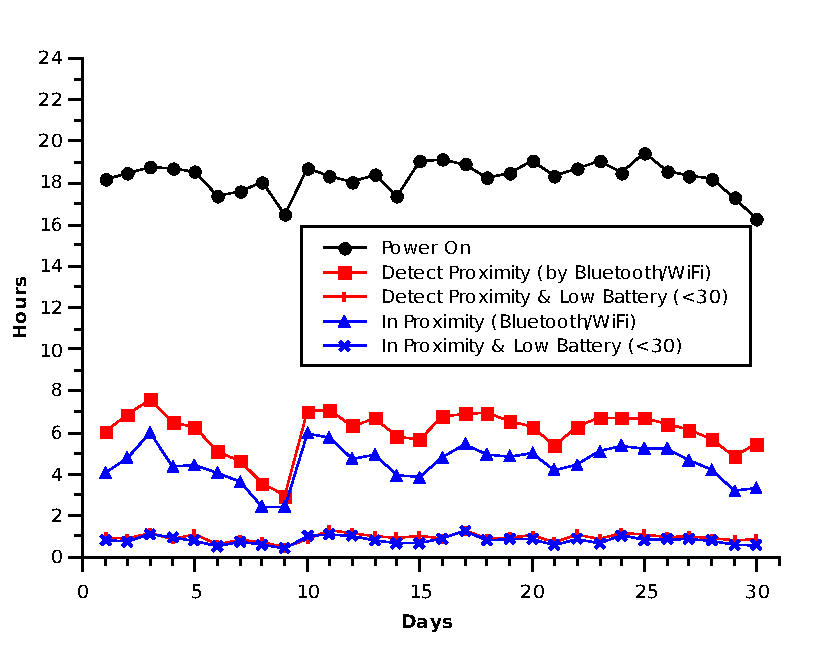
\includegraphics[width=3.5in]{graphs/battery.pdf}}
\caption{Average Daily Low Residual Battery Time in April 2012} 
\label{fig:battery}
\end{figure} 

\subsubsection*{Evaluating Availability} 

To summarize, we conclude availability of opportunistic communication with a brief discussion of metrics used to evaluate availability.
\begin{itemize}
	\item Sufficient Signal: While the use of all available proximity potentially may be of interest, only useable mobile-to-mobile links are of interest.  An explicit filter likely unique to each particular handset or device should be employed.  
	\item Symmetry: Filtering the data further, agents monitoring the signal strength on both sides of the dyadic pair can assess if symmetry exists both with respect to detection ($MN_i$ detects $MN_j$, vice versa) and sufficient signal strength.  
	\item Diversity: When there are more than one relaying nodes nearby, it is easier for the device to choose one of the most appropriate nodes with the consideration of benefits on both sides. 
	\item Residual Battery: As an important criterion for relaying selection in various relaying protocol, battery of mobile devices is essential for availability. When the residual battery of mobile devices is low, it is difficult for the devices to do opportunistic communication.  
\end{itemize} 

\subsection{Prevalence}\label{sec:prevalence}
Availability analysis exhibits the possibility to detect other devices in proximity. A more important question is to what extent such opportunistic communication opportunities exist in practice.  We begin with the most basic question with regards to the prevalence of discoverable Bluetooth devices and further refine our queries to explore various aspects of prevalence through the Prevalence criterion of the APSR framework.  We posit several questions that include: (1) the extent to which discoverable Bluetooth devices exist, (2) the extent to which WiFi proximity exist, (3) and the extent to which diurnal (daily) patterns play a role in discoverable devices.  We further continue the explorations examining the prevalence of proximity to determine if the prevalence of such opportunities are still useful, namely (1) are such opportunities only available when there is no traffic and (2) how frequent do opportunities exist to augment access to `better' wireless channels (ex. WiFi).   


\subsubsection*{Time in Proximity}
Based on the 15 months data, Figure~\ref{fig:bluetooth} illustrates the average weekly Bluetooth proximity percentage with different restrictions across the study period.  Various periods of interest representing various break periods are labeled in the graph. Further restrictions are placed on the data to filter for `good RSSI' and candidates for opportunistic communications to exist only within the project (study).   Notably, when completely unrestricted opportunities exist on the average of nearly 60\% of the time when on campus, falling only slightly when good signal strength is added as a restriction.  Even intra-study opportunities are quite prolific despite the fact that the 200 study participants represent less than one tenth of the freshmen class and less than 2.5\% of the overall university student population.With the threshold of -80dBm for the `Good RSSI', there still exists more than 50\% of the time slots, a fairly insubstantial drop from the raw detected Bluetooth devices. The slight drop from the fall of 2011 to the fall of 2012 can largely be attributed to students joining their respective majors and having less shared coursework versus their freshmen year.  Moreover, we compare Bluetooth proximity with and without consideration of symmetry. Similarly as the results in Figure~\ref{fig:daily_symmetric}, the one third drop rate due to asymmetry is quite stable across the study.  Although the lack of symmetry does temper the earlier findings of prevalence, we note that Bluetooth is most appropriately viewed as a floor for potential interactions.  The potential for asymmetry though between nodes does represent a consideration that merits further attention.  

\begin{figure}[tbp]
\centering 
{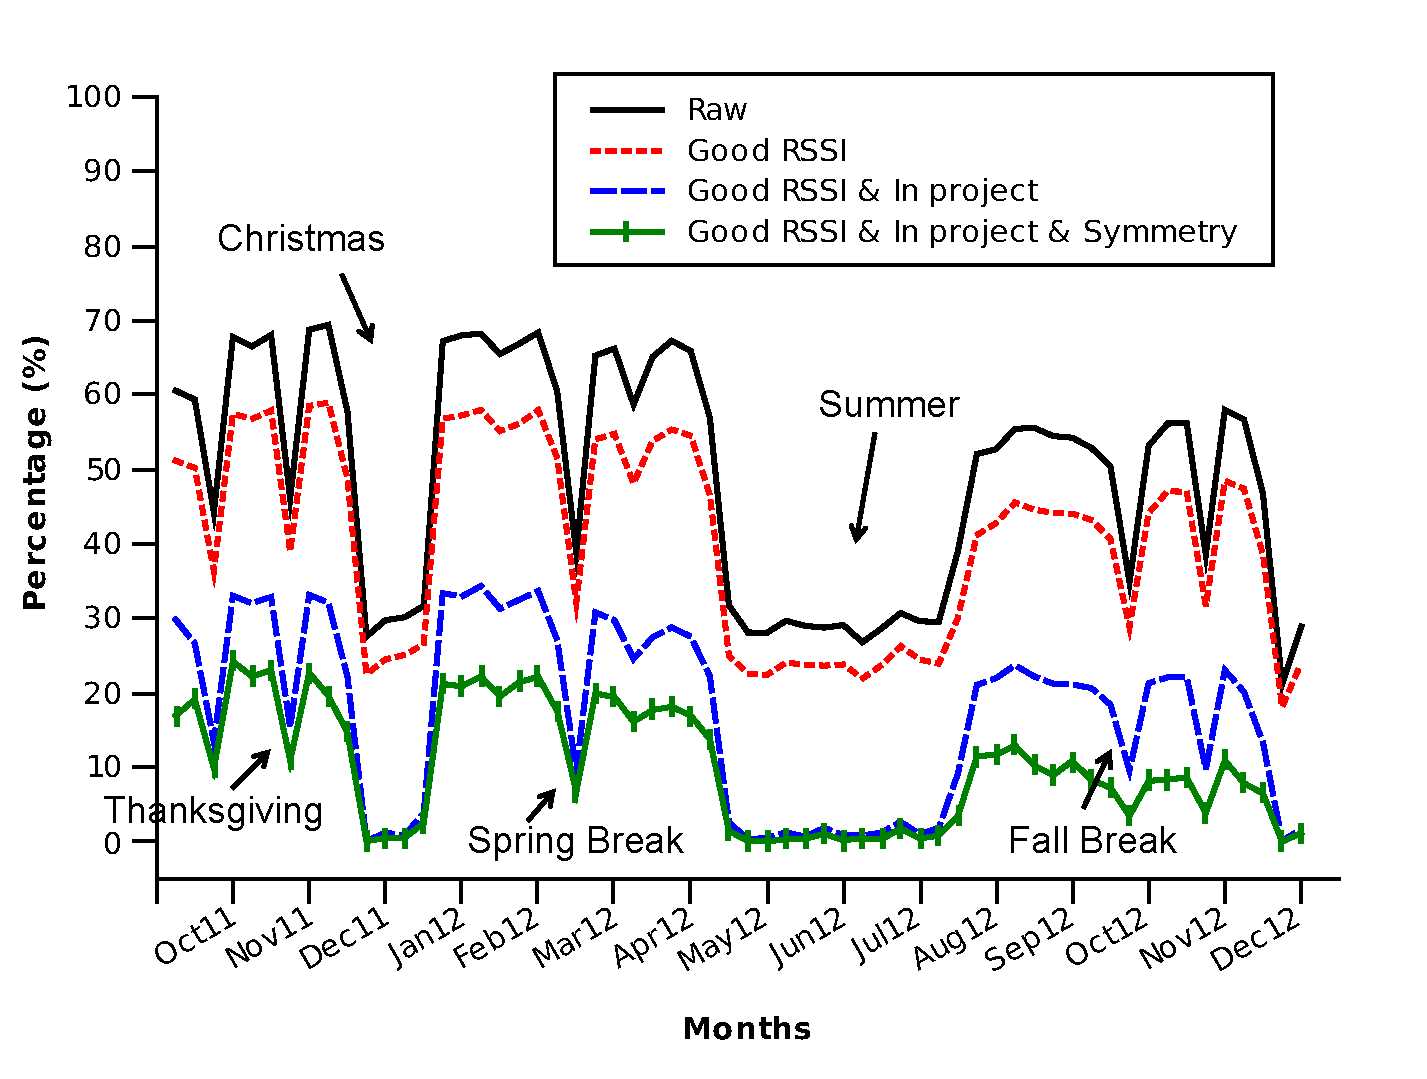
\includegraphics[width=3.5in]{graphs/weekly_bluetooth_with_symmetry_tag.pdf}}
\caption{Bluetooth Proximity with Different Restrictions} 
\label{fig:bluetooth}
\end{figure} 

Given that the students were selected from a core group of six dormitories, a natural skepticism should emerge from the data with regards to the diurnal effects of proximity, namely proximity does little good if it only occurs at night when the phone is not otherwise being used (ex. sleeping in the dorm room).  Hence, we analyze the diurnal distribution of Bluetooth proximity by dividing one day into three parts: day time (8am to 4pm), night time (4pm to 12am) and sleep (12am to 8am). In this way, we are able to investigate the impacts of time durations on such proximity. Figure~\ref{fig:diurnal} shows the diurnal distribution with the twin restrictions of good RSSI and intra-study detected proximity only. The daytime proximity percentage from 8am to 4pm is larger than the value during nighttime and almost equal to the value of sleep time.  The separation from in the fall of 2012 largely follows the classroom / major separation as noted in the raw and restricted graphs. 

\begin{figure}[tbp]
\centering 
{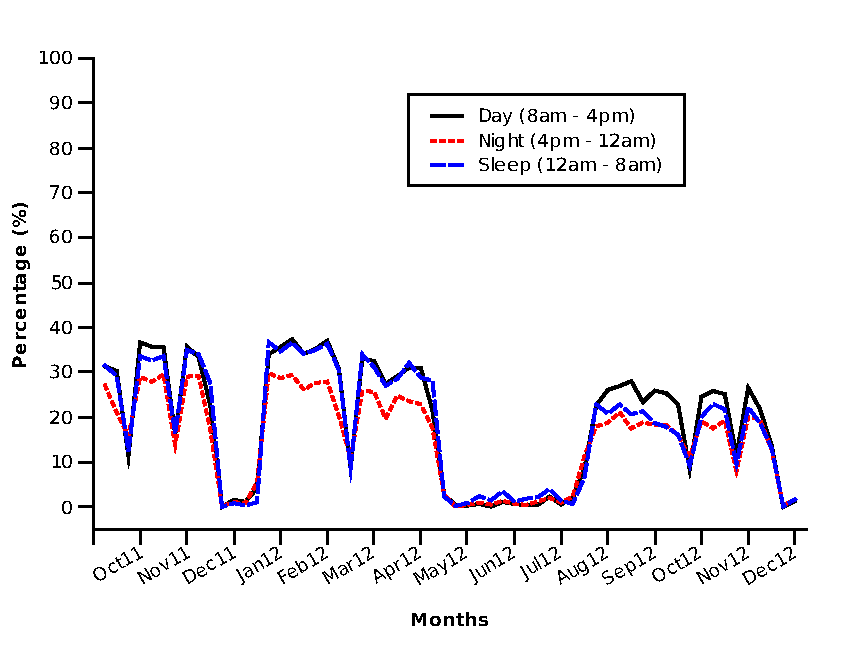
\includegraphics[width=3.5in]{graphs/weekly_bluetooth_diurnal.pdf}}
 \caption{Diurnal Distribution of \\Bluetooth Proximity} 
\label{fig:diurnal}
\end{figure} 

Beyond coarse diurnal metrics, significant day of week effects can also exist. Course patterns can vary dramatically between the Monday / Wednesday / Friday courses and Tuesday / Thursday courses.  Similarly, weekends are much more likely to be quite diverse from normal weekday patterns.  Figure~\ref{fig:diurnal_april} shows the daily Bluetooth proximity and diurnal distribution in April 2012 for a more detailed comparisons among the weekdays with each respective Saturday noted on the x axis. The peak values always appear at the beginning of the week and decrease slowly during the week. During the Easter holiday (April 6th - April 9th), the opportunities for proximity shrink dramatically as the students travel home for Easter break. Meanwhile, more Bluetooth proximity appeared in the later hours (broadly defined as sleep time) than daytime hours during weekend which indicates the participants spent more time in closer proximity to others during those time periods largely as a byproduct of social relationships. 
